\section{Dreiachsiger Spannungszustand\label{spannung:section:Dreiachsiger_Spannungszustand}}
\rhead{Dreiachsiger Spannungszustand}
Durch komplexe Spannungsausbreitungen im Boden entstehen im 3D-Spannungszustand unterschiedliche Normal- und Schubspannungen.
\begin{figure}
	\centering
	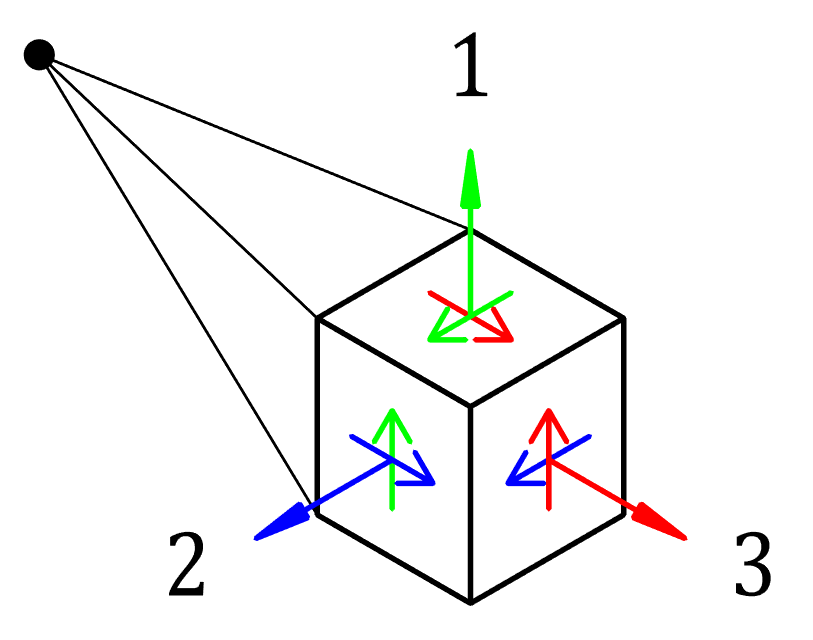
\includegraphics[width=0.30\linewidth,keepaspectratio]{papers/spannung/Grafiken/infinitesimalerWuerfel.png}
	\caption{Beispiel eines Spannungszustandes; Vergrösserung eines infinitesimalen Bodenteilchens}
	\label{fig:infinitesimalerWuerfel}
\end{figure}
Ein Tensor 0.~Stufe, sprich ein Skalar, kann lediglich den 1D-Spannungszustand beschreiben.
Um den 3D-Spannungszustand als ein mathematisches Objekt darstellen zu können, wird ein Tensor 2.~Stufe, sprich eine Matrix, eingesetzt.
Die Spannungen sind durch die zwei Indizes
\(
i, j\in\left\{1, 2, 3\right\}
\)
definiert.
Daher ergeben sich die $9$ Spannungen.
Die nachfolgenden Zusammenhänge sind in \cite{spannung:Voigtsche-Notation} beschrieben.
Dieser Spannungstensor kann schliesslich mit $3^2$ Einträgen als $3\times3$ Matrix mit
\[
\overline{\sigma}
=
\sigma_{ij}
=
\begin{pmatrix}
	\sigma_{11} & \sigma_{12} & \sigma_{13} \\ 
	\sigma_{21} & \sigma_{22} & \sigma_{23} \\
	\sigma_{31} & \sigma_{32} & \sigma_{33}
\end{pmatrix}
\]
dargestellt werden und beschreibt somit den gesamten Spannungszustand.
Die Dehnungen wirken in die gleichen Richtungen wie die korrespondierenden Spannungen und sind durch die zwei Indizes
\(
k, l\in\left\{1, 2, 3\right\}
\)
definiert.
Der Dehnungstensor ist ebenfalls ein Tensor 2.~Stufe und kann somit auch als $3\times3$ Matrix mit
\[
\overline{\varepsilon}
=
\varepsilon_{kl}
=
\begin{pmatrix}
	\varepsilon_{11} & \varepsilon_{12} & \varepsilon_{13} \\ 
	\varepsilon_{21} & \varepsilon_{22} & \varepsilon_{23} \\
	\varepsilon_{31} & \varepsilon_{32} & \varepsilon_{33}
\end{pmatrix}
\]
dargestellt werden und beschreibt den gesamten Dehnungszustand.

Der Spannungs- und Dehnungstensor 2.~Stufe kann je in einen Tensor 1.~Stufe überführt werden, welcher ein Spaltenvektor ist.
Man darf Zeile um Zeile in eine Spalte notieren, sodass es einen Spaltenvektor ergibt.
So ergibt sich der Spannungsvektor

\[
\overline{\sigma}
=
\sigma_{ij}
=
\begin{pmatrix}
	\sigma_{11} & \sigma_{12} & \sigma_{13} \\ 
	\sigma_{21} & \sigma_{22} & \sigma_{23} \\
	\sigma_{31} & \sigma_{32} & \sigma_{33}
\end{pmatrix}
\qquad
\Rightarrow
\qquad
\vec{\sigma}
=
\begin{pmatrix}
	\sigma_{11}\\
	\sigma_{12}\\
	\sigma_{13}\\
	\sigma_{21}\\
	\sigma_{22}\\
	\sigma_{23}\\
	\sigma_{31}\\
	\sigma_{32}\\
	\sigma_{33}
\end{pmatrix}
\]
und der Dehnungsvektor
\[
\overline{\varepsilon}
=
\varepsilon_{kl}
=
\begin{pmatrix}
	\varepsilon_{11} & \varepsilon_{12} & \varepsilon_{13} \\ 
	\varepsilon_{21} & \varepsilon_{22} & \varepsilon_{23} \\
	\varepsilon_{31} & \varepsilon_{32} & \varepsilon_{33}
\end{pmatrix}
\qquad
\Rightarrow
\qquad
\vec{\varepsilon}
=
\begin{pmatrix}
	\varepsilon_{11} \\
	\varepsilon_{12} \\
	\varepsilon_{13} \\
	\varepsilon_{21} \\
	\varepsilon_{22} \\
	\varepsilon_{23} \\
	\varepsilon_{31} \\
	\varepsilon_{32} \\
	\varepsilon_{33}
\end{pmatrix}
.
\]
Um die Beziehung von Spannung und Dehnung, welche mit Tensoren 2.~Stufe ausgedrückt werden, zu beschreiben, wird ein Elastizitätstensor 4.~Stufe benötigt.
\index{Elastizitätstensor}%
Dieser ist im 1D-Spannungszustand ein Tensor 0.~Stufe und somit ein Skalar, der Elastizitätsmodul $E$.

Dieser Elastizitätstensor 4.~Stufe kann als Tensor 2.~Stufe, sprich als Matrix, dargestellt werden.
So wird die Spannungsgleichung stark vereinfacht, da nun eine Matrix auf einen Vektor operiert.
Dieser Tensor muss für eine Spannung jeden Einfluss aus allen $9$ Dehnungen mit Konstanten erfassen.
Dies bedeutet um eine von $9$ Spannungen berechnen zu können müssen alle $9$ Dehnung mit unterschiedlichen Faktoren summiert werden.
Es ergeben sich $9^2$ Einträge, welches mit den vier Indizes
\(
i, j, k, l\in\left\{1, 2, 3\right\}
,
\)
die zueinander verknüpft werden müssen, zu begründen ist.
Es ergeben sich $3^4$ Einträge, sprich eine $9\times9$ Matrix, welche allgemein
\[
\overline{\overline{C}}
=
C_{ijkl}
=
\begin{pmatrix}
C_{1111} & C_{1112} & C_{1113} & C_{1121} & C_{1122} & C_{1123} & C_{1131} & C_{1132} & C_{1133} \\
C_{1211} & C_{1212} & C_{1213} & C_{1221} & C_{1222} & C_{1223} & C_{1231} & C_{1232} & C_{1233} \\
C_{1311} & C_{1312} & C_{1313} & C_{1321} & C_{1322} & C_{1323} & C_{1331} & C_{1332} & C_{1333} \\
C_{2111} & C_{2112} & C_{2113} & C_{2121} & C_{2122} & C_{2123} & C_{2131} & C_{2132} & C_{2133} \\
C_{2211} & C_{2212} & C_{2213} & C_{2221} & C_{2222} & C_{2223} & C_{2231} & C_{2232} & C_{2233} \\
C_{2311} & C_{2312} & C_{2313} & C_{2321} & C_{2322} & C_{2323} & C_{2331} & C_{2332} & C_{2333} \\
C_{3111} & C_{3112} & C_{3113} & C_{3121} & C_{3122} & C_{3123} & C_{3131} & C_{3132} & C_{3133} \\
C_{3211} & C_{3212} & C_{3213} & C_{3221} & C_{3222} & C_{3223} & C_{3231} & C_{3232} & C_{3233} \\
C_{3311} & C_{3312} & C_{3313} & C_{3321} & C_{3322} & C_{3323} & C_{3331} & C_{3332} & C_{3333}
\end{pmatrix}
\]
geschrieben werden kann.
Die allgemeine Spannungsgleichung lautet nun:
\[
\vec\sigma
=
\overline{\overline{C}}\cdot\vec{\varepsilon}
.
\]
Sie kann ebenfalls als Indexnotation
\[
\sigma_{ij}
=
\sum_{k=1}^3
\sum_{l=1}^3
C_{ijkl}\cdot\varepsilon_{kl}
\]
geschrieben werden.
Der Elastizitätstensor muss für isotrope Materialien zwingend symmetrisch sein.
\index{isotrop}%
Folglich gilt:
\[
\overline{\overline{C}}
=
\overline{\overline{C}}~^{T}
.
\]

Die Konstanten $C$ werden nun nach dem Hook'schen Gesetz mit Hilfe des Elastizitätsmoduls $E$ definiert.
Da dieser Modul durch die eindimensionale Betrachtung definiert ist,
muss für die dreidimensionale Betrachtung eine weitere Kennzahl eingeführt werden.
Dies ist die Querdehnungszahl $\nu$ (auch Poisson-Zahl), welche durch
\index{Querdehnungszahl}%
\index{Poisson-Zahl}%
\[
\nu
=
\frac{\varepsilon_q}{\varepsilon}
=
\frac{\Delta b}{b_0}
\]
und
\begin{align*}
	\varepsilon     &= \text{Längsdehnung [$-$]} \\
	\varepsilon_q   &= \text{Querdehnung [$-$]}
\end{align*}
definiert ist. Trägt man die Konstanten in die Matrix ein, ergibt sich
\[
\begin{pmatrix}
	\sigma_{11}\\
	\sigma_{12}\\
	\sigma_{13}\\
	\sigma_{21}\\
	\sigma_{22}\\
	\sigma_{23}\\
	\sigma_{31}\\
	\sigma_{32}\\
	\sigma_{33}
\end{pmatrix}
=
\frac{E}{(1+\nu)(1-2\nu)}
\begin{pmatrix}
	1-2\nu &          0 &          0 &          0 &    \nu &          0 &          0 &          0 & \nu   \\
	     0 &\frac{1}{4} &          0 &\frac{1}{4} &      0 &          0 &          0 &          0 & 0     \\
	     0 &          0 &\frac{1}{4} &          0 &      0 &          0 &\frac{1}{4} &          0 & 0     \\
	     0 &\frac{1}{4} &          0 &\frac{1}{4} &      0 &          0 &          0 &          0 & 0     \\
	   \nu &          0 &          0 &          0 & 1-2\nu &          0 &          0 &          0 & \nu   \\
  	     0 &          0 &          0 &          0 &      0 &\frac{1}{4} &          0 &\frac{1}{4} & 0     \\
	     0 &          0 &\frac{1}{4} &          0 &      0 &          0 &\frac{1}{4} &          0 & 0     \\
	     0 &          0 &          0 &          0 &      0 &\frac{1}{4} &          0 &\frac{1}{4} & 0     \\
	   \nu &          0 &          0 &          0 &    \nu &          0 &          0 &          0 & 1-2\nu
\end{pmatrix}
\begin{pmatrix}
	\varepsilon_{11} \\
	\varepsilon_{12} \\
	\varepsilon_{13} \\
	\varepsilon_{21} \\
	\varepsilon_{22} \\
	\varepsilon_{23} \\
	\varepsilon_{31} \\
	\varepsilon_{32} \\
	\varepsilon_{33}
\end{pmatrix}
.
\]
Die Normalspannung $\sigma_{22}$ lässt sich zum Beispiel als
\[
\sigma_{22}
=
\frac{E\cdot\nu}{(1+\nu)(1-2\nu)}\cdot\varepsilon_{11}+\frac{E}{(1+\nu)}\cdot\varepsilon_{22}+\frac{E\cdot\nu}{(1+\nu)(1-2\nu)}\cdot\varepsilon_{33}
\]
berechnen.

\section{Reduzierte Spannungs- und Dehnungsgleichungen}
\rhead{Reduzierte Spannungs- und Dehnungsgleichungen}
Man betrachte nun die Eigenschaften des Elastizitätstensors.
Dieser ist quadratisch und symmetrisch, die verschiedenen Einträge wechseln sich aber miteinander ab.
Es ergeben sich keine Blöcke mit einheitlichen Einträgen.

Allerdings weiss man, dass im isotropen Boden der Spannungs-, Dehnungs- und daher auch der Elastizitätstensor symmetrisch sind.
Wäre dem nicht so, würde sich das Material je nach Richtung unterschiedlich elastisch verhalten.
Diese Symmetrie setzt daher voraus, dass
\[
\sigma_{12}
=
\sigma_{21}
,
\qquad
\sigma_{13}
=
\sigma_{31}
,
\qquad
\sigma_{23}
=
\sigma_{32}
\]
und folglich auch
\[
\varepsilon_{12}
=
\varepsilon_{21}
,
\qquad
\varepsilon_{13}
=
\varepsilon_{31}
,
\qquad
\varepsilon_{23}
=
\varepsilon_{32}
\]
gilt.
Diese Eigenschaft wird durch die Voigt'sche Notation \cite{spannung:Voigtsche-Notation} ausgenutzt, um die Gleichung vereinfachen zu können.
\index{Voigt'sche Notation}%
Durch diese Symmetrie gilt
\[
\overline{\sigma}
=
\begin{pmatrix}
	\sigma_{11} & \sigma_{12} & \sigma_{13} \\ 
	\sigma_{21} & \sigma_{22} & \sigma_{23} \\
	\sigma_{31} & \sigma_{32} & \sigma_{33}
\end{pmatrix}
=
\begin{pmatrix}
	\sigma_{11} & \sigma_{12} & \sigma_{13} \\ 
  	            & \sigma_{22} & \sigma_{23} \\
	 \text{sym} &             & \sigma_{33} 
\end{pmatrix}
\qquad
\Rightarrow
\qquad
\vec{\sigma}
=
\begin{pmatrix}
    \sigma_{11}\\
	\sigma_{22}\\
	\sigma_{33}\\
	\sigma_{23}\\
	\sigma_{13}\\
	\sigma_{12}
\end{pmatrix}
\]
und entsprechend
\[
\overline{\varepsilon}
=
\begin{pmatrix}
	\varepsilon_{11} & \varepsilon_{12} & \varepsilon_{13} \\ 
	\varepsilon_{21} & \varepsilon_{22} & \varepsilon_{23} \\
	\varepsilon_{31} & \varepsilon_{32} & \varepsilon_{33}
\end{pmatrix}
=
\begin{pmatrix}
	\varepsilon_{11} & \varepsilon_{12} & \varepsilon_{13} \\ 
	                 & \varepsilon_{22} & \varepsilon_{23} \\
	\text{sym}       &                  & \varepsilon_{33}
\end{pmatrix}
\qquad
\Rightarrow
\qquad
\vec{\varepsilon}
=
\begin{pmatrix}
	\varepsilon_{11} \\
	\varepsilon_{22} \\
	\varepsilon_{33} \\
	\varepsilon_{23} \\
	\varepsilon_{13} \\
	\varepsilon_{12}
\end{pmatrix}
.
\]

Aus den Vereinfachungen der Voigt'schen Notation lassen sich die Spannungs- und Dehnungstensoren als Spaltenvektoren mit je sechs Einträgen darstellen.
Der Elastizitätstensor kann entsprechend auf eine $6\times6$ Matrix reduziert werden.
Es lässt sich nun eine reduzierte allgemeine Spannungsgleichung mit
\[
\vec{\sigma}
=
\overline{\overline{C}}\cdot\vec{\varepsilon}
\]
beziehungsweise
\[
\begin{pmatrix}
	\sigma_{11} \\
	\sigma_{22} \\
	\sigma_{33} \\
	\sigma_{23} \\
	\sigma_{13} \\
	\sigma_{12}
\end{pmatrix}
=
%\left(
%\begin{array}{ccc|ccc}
\begin{pmatrix}
	C_{1111} & C_{1122} & C_{1133} & C_{1123} & C_{1113} & C_{1112} \\
	C_{2211} & C_{2222} & C_{2233} & C_{2223} & C_{2213} & C_{2212} \\
	C_{3311} & C_{3322} & C_{3333} & C_{3323} & C_{3313} & C_{3312} \\
%\hline
	C_{2311} & C_{2322} & C_{2333} & C_{2323} & C_{2313} & C_{2312} \\
	C_{1311} & C_{1322} & C_{1333} & C_{1323} & C_{1313} & C_{1312} \\
	C_{1211} & C_{1222} & C_{1233} & C_{1223} & C_{1213} & C_{1212}
\end{pmatrix}
%\end{array}
%\right)
\begin{pmatrix}
	\varepsilon_{11} \\
	\varepsilon_{22} \\
	\varepsilon_{33} \\
	\varepsilon_{23} \\
	\varepsilon_{13} \\
	\varepsilon_{12}
\end{pmatrix}
\]
beschreiben.
Die Spannung $\sigma_{11}$ beispielsweise erhält man, wenn man die sechs Produkte aus den Konstanten $C$ und Dehnungen $\varepsilon$ summiert.
Die Symmetrieeigenschaft des Elastizitätstensors bleibt auch hier erhalten.
Somit lässt sich die reduzierte allgemeine Spannungsgleichung mit

\[
\begin{pmatrix}
	\sigma_{11} \\
	\sigma_{22} \\
	\sigma_{33} \\
	\sigma_{23} \\
	\sigma_{13} \\
	\sigma_{12}
\end{pmatrix}
=
\begin{pmatrix}
	  C_{1111} & C_{1122} & C_{1133} & C_{1123} & C_{1113} & C_{1112} \\
	           & C_{2222} & C_{2233} & C_{2223} & C_{2213} & C_{2212} \\
	           &          & C_{3333} & C_{3323} & C_{3313} & C_{3312} \\ 
	           &          &          & C_{2323} & C_{2313} & C_{2312} \\ 
               &          &          &          & C_{1313} & C_{1312} \\
    \text{sym} &          &          &          &          & C_{1212} 
\end{pmatrix}
\begin{pmatrix}
	\varepsilon_{11} \\
	\varepsilon_{22} \\
	\varepsilon_{33} \\
	\varepsilon_{23} \\
	\varepsilon_{13} \\
	\varepsilon_{12}
\end{pmatrix}
\]
beschreiben.
Die Konstanten $C$ werden wieder nach dem Hook'schen Gesetz definiert.
Dies ergibt die Spannungsgleichung, welche weit möglichst vereinfacht ist:
\begin{equation}
\begin{pmatrix}
	\sigma_{11}\\
	\sigma_{22}\\
	\sigma_{33}\\
	\sigma_{23}\\
	\sigma_{13}\\
	\sigma_{12}
\end{pmatrix}
=
\frac{E}{(1+\nu)(1-2\nu)}
\left(
\begin{array}{ccc|ccc}
%\begin{pmatrix}
	1- 2\nu & \nu     & \nu     & 0           & 0           & 0\\
	    \nu & 1- 2\nu & \nu     & 0           & 0           & 0\\
        \nu & \nu     & 1- 2\nu & 0           & 0           & 0\\
\hline
          0 & 0       & 0       & \frac{1}{2} & 0           & 0\\
          0 & 0       & 0       & 0           & \frac{1}{2} & 0\\
          0 & 0       & 0       & 0           & 0           & \frac{1}{2}
%\end{pmatrix}
\end{array}
\right)
\begin{pmatrix}
	\varepsilon_{11}\\
	\varepsilon_{22}\\
	\varepsilon_{33}\\
	\varepsilon_{23}\\
	\varepsilon_{13}\\
	\varepsilon_{12}
\end{pmatrix}
.
\label{spannung:Spannungsgleichung}
\end{equation}

Im Elastizitätstensor fallen zwei $3\times3$ Blöcke auf, welche nur Einträge mit $0$ haben. Der Tensor besagt also,
dass diese jeweiligen Dehnungen keinen Einfluss auf unsere Spannung haben.
Man sieht nun auch ganz gut, dass sich im Vergleich zu der allgemeinen Spannungsgleichung die Einträge verschoben haben.
Da nach Voigt zuerst die Normalspannungen und anschliessend die Schubspannungen notiert worden sind, ergeben sich die  $3\times3$ Blöcke.

Man betrachte als Beispiel die Berechnung von $\sigma_{33}$.
Es ist ersichtlich, dass die Schubdehnungen keinen Einfluss auf $\sigma_{33}$ haben.
Der Einfluss der zu $\sigma_{33}$ äquivalenten Dehnung $\varepsilon_{33}$ hat den grössten Einfluss.
Die anderen Normalspannungen $\sigma_{11}$ und $\sigma_{22}$ haben einen unter anderem mit $\nu$ korrigierten Einfluss.

Von  $\overline{\overline{C}}$ bildet man die inverse Matrix $\overline{\overline{C}}\mathstrut^{-1}$, mithilfe des Gauss-Jordan-Algorithmus, um die Gleichung umstellen zu können.
\index{Gauss-Algorithmus}%
Durch einige Berechnungsschritte erhält man die Dehnungsgleichung:

\[
\vec{\varepsilon}
=
\overline{\overline{C}}\mathstrut^{-1}\cdot \vec{\sigma}
\]

\[
\begin{pmatrix}
	\varepsilon_{11}\\
	\varepsilon_{22}\\
	\varepsilon_{33}\\
	\varepsilon_{23}\\
	\varepsilon_{13}\\
	\varepsilon_{12}
\end{pmatrix}
=
\frac{1}{E}
\left(
\begin{array}{ccc|ccc}
%\begin{pmatrix}
	   1 & -\nu & -\nu & 0      & 0      & 0     \\
	-\nu &    1 & -\nu & 0      & 0      & 0     \\
	-\nu & -\nu &    1 & 0      & 0      & 0     \\
\hline
 	   0 &    0 &    0 & 2+2\nu & 0      & 0     \\
	   0 &    0 &    0 &      0 & 2+2\nu & 0     \\
	   0 &    0 &    0 &      0 & 0      & 2+2\nu
%\end{pmatrix}
\end{array}
\right)
\begin{pmatrix}
	\sigma_{11}\\
	\sigma_{22}\\
	\sigma_{33}\\
	\sigma_{23}\\
	\sigma_{13}\\
	\sigma_{12}
\end{pmatrix}
.
\]
Die zwei $3\times3$ Blöcke links unten und rechts oben sind folglich noch vorhanden.
Um wieder die Einflüsse der Parameter veranschaulichen zu können berechnet man die Dehnung
\[
\varepsilon_{22}
=
\frac{1}{E}\sigma_{22} - \frac{\nu}{E}\sigma_{11} - \frac{\nu}{E}\sigma_{33}
=
\frac{1}{E}\cdot(\sigma_{22}-\nu\cdot\sigma_{11}-\nu\cdot\sigma_{33})
.
\]
Diese hängt wieder am meisten von $\sigma_{22}$ ab.
Ist die Querdehnung $\nu$ grösser, so wird die Dehnung $\varepsilon_{22}$ reduziert.
Bei inkompressiblen Medien, bei welchen keine Dehnungen und nur identische Normalspannungen auftreten können, ist folglich $\nu=\frac12$.
